
\subsection{Homotopic maps}
\label{sec:Homotopic-maps}

By a \nomen{loop} we mena a continuous map $\alpha:I\to X$ such that
$\alpha(0)=\alpha(1)$. We can view is also as a continuous map
$\alpha:S^1 \to X$. It is said to be based at the point
$\alpha(0)$. Two loops $\alpha$ and $\beta$ with the same \nomen{base
point} can be multiplied, and their product is defined on page 87.
A visualization of $\alpha\cdot\beta$ is here:
\begin{figure}[H]
    \centering
    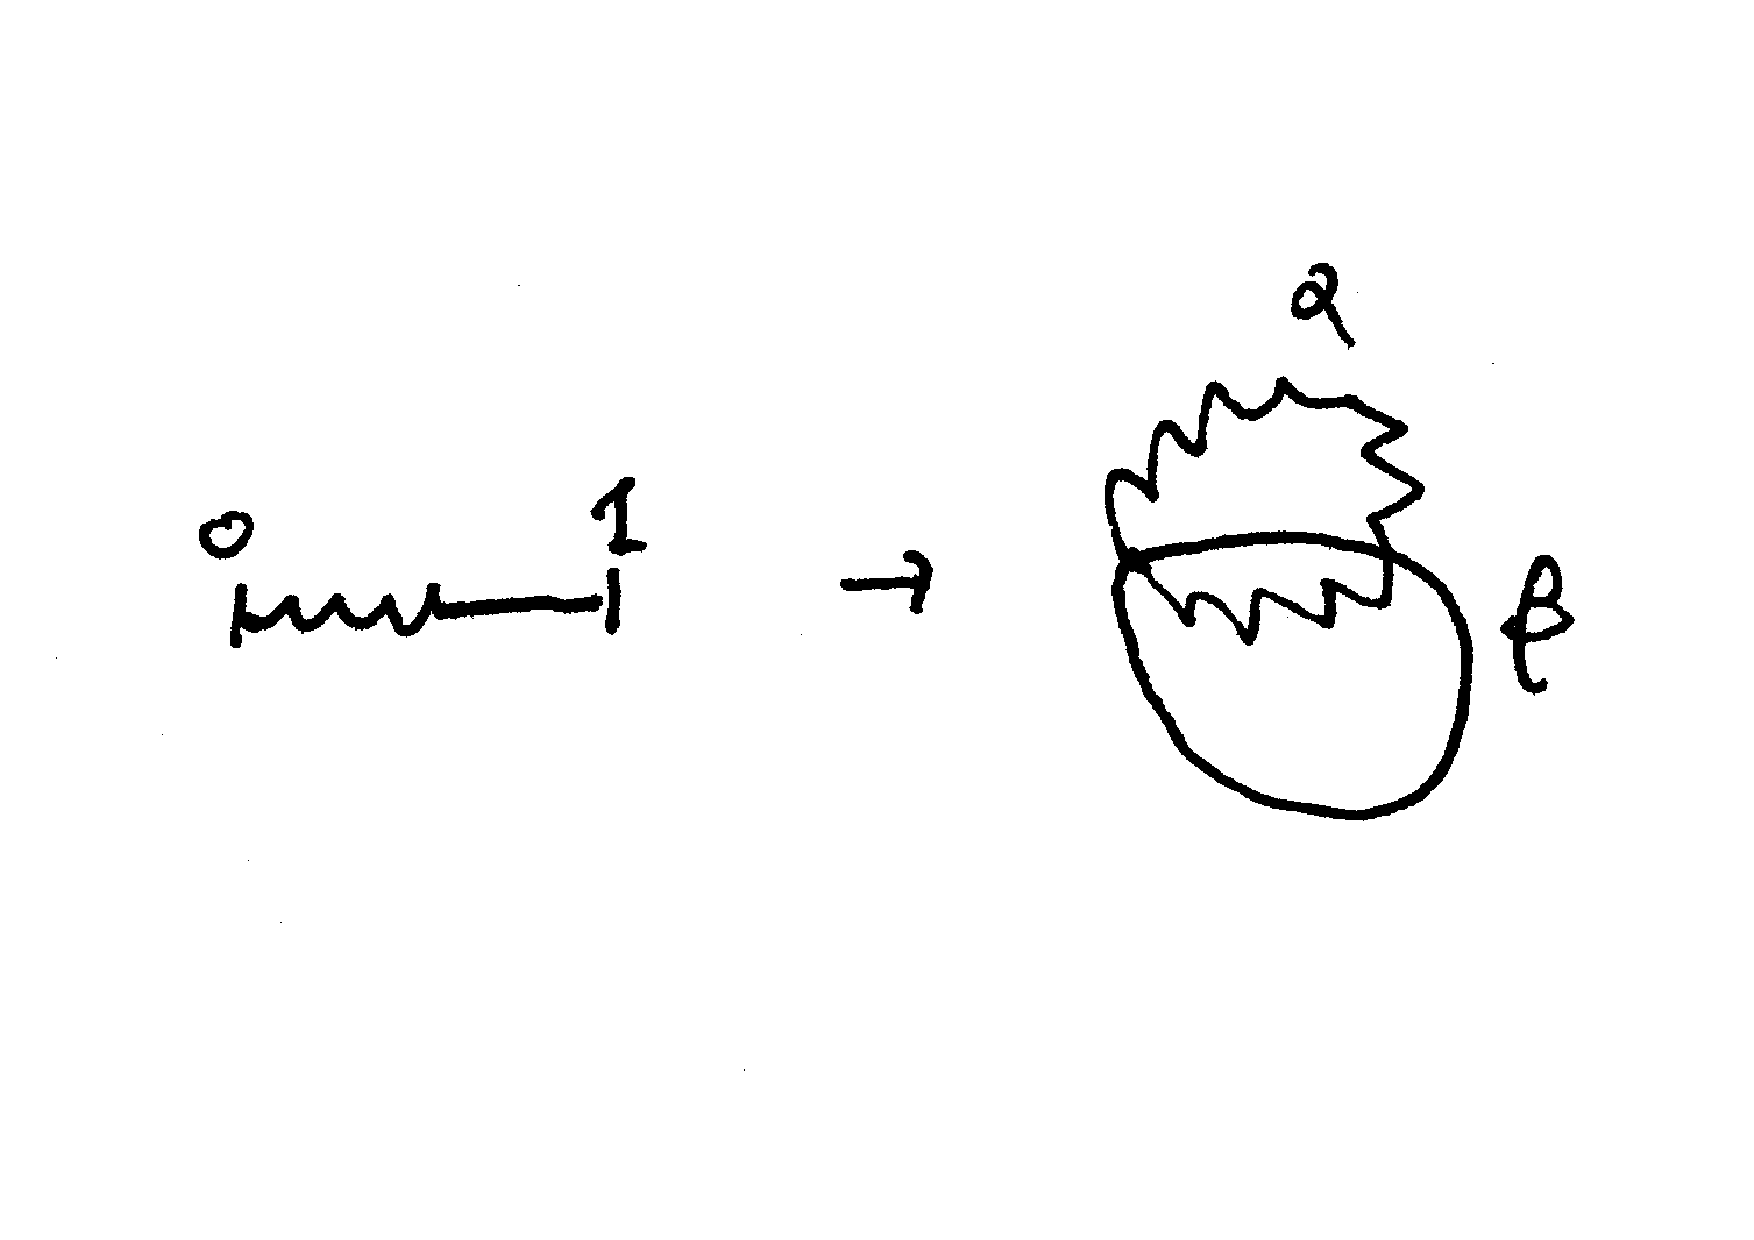
\includegraphics[width=0.4\linewidth]{pics/multiply-loops.pdf}
    \caption{Multiply loops}
\end{figure}
But this product is not sufficient to become a group. At least, the
multiplication is not associative:
\begin{figure}[H]
    \centering
    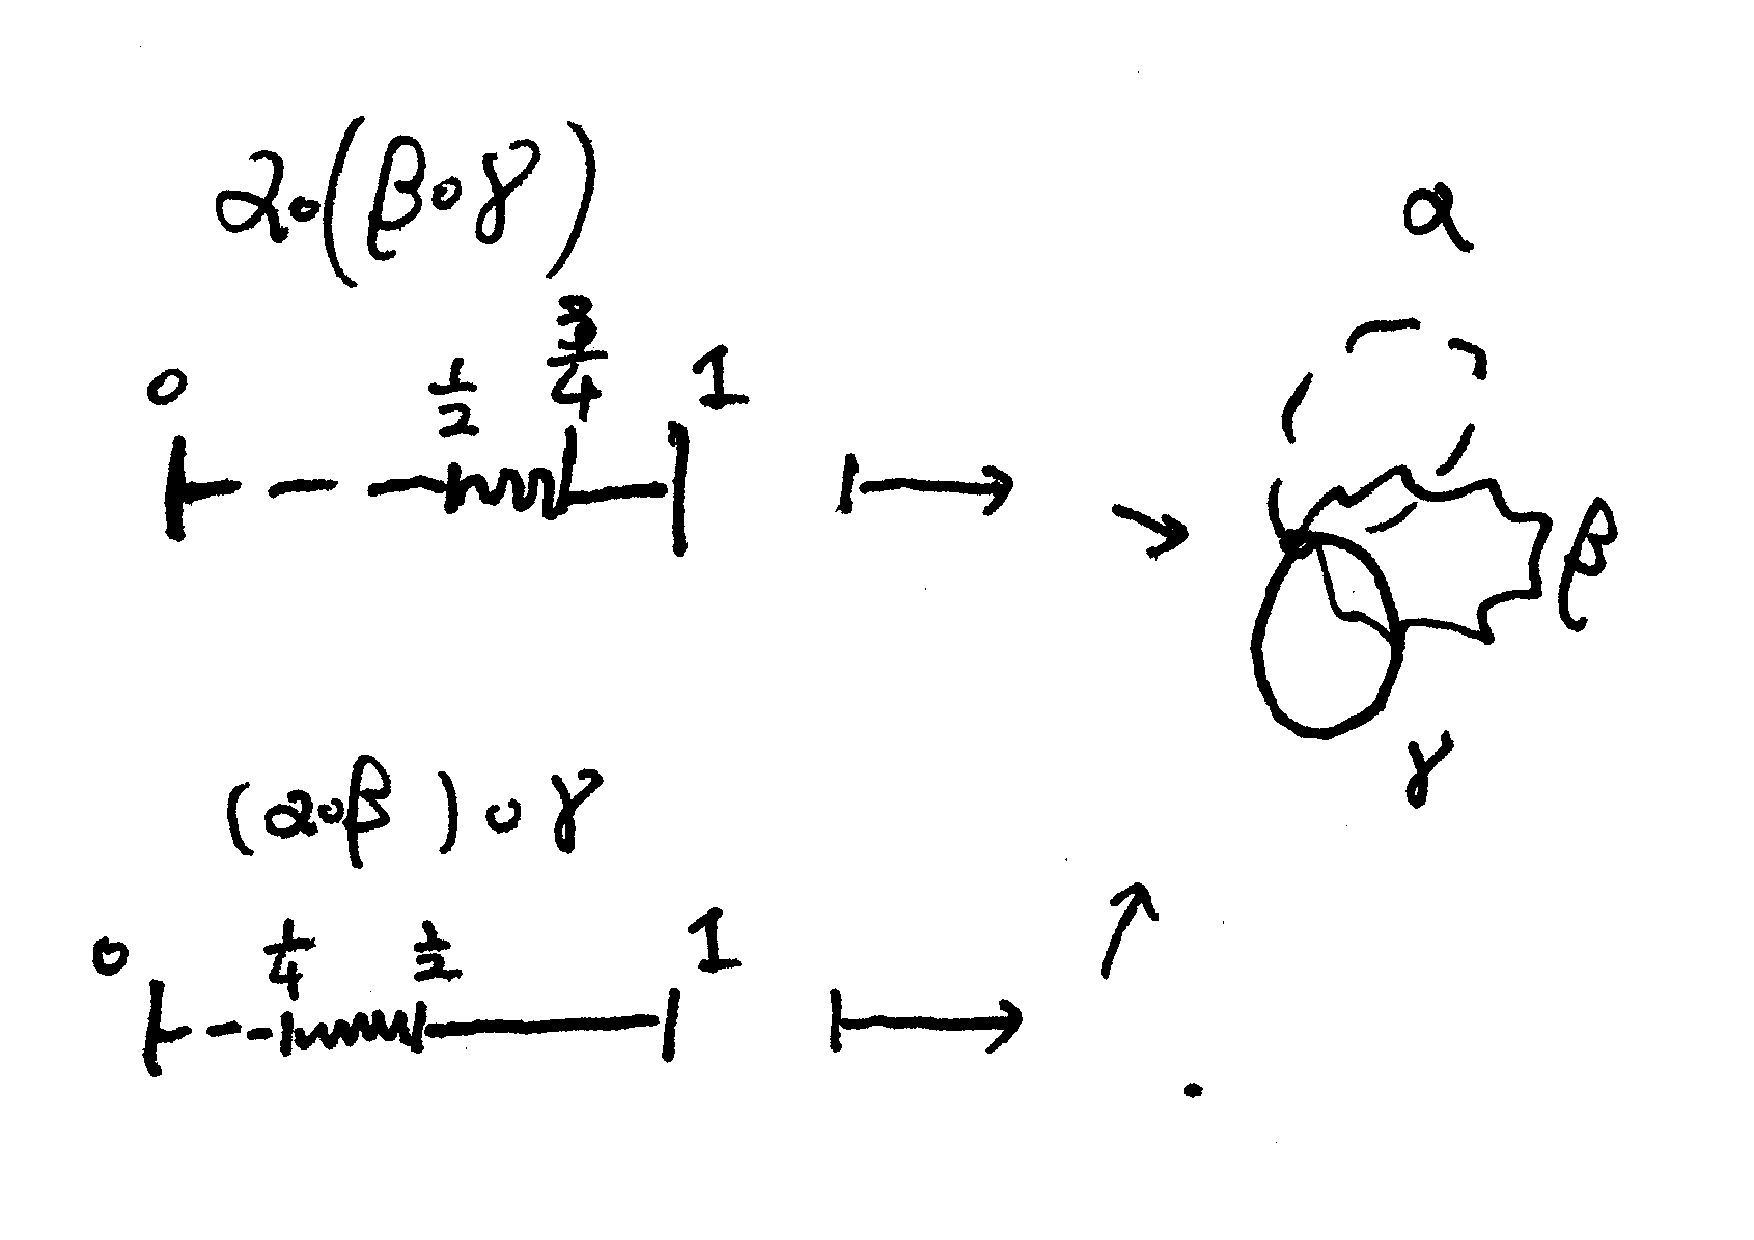
\includegraphics[width=0.6\linewidth]{pics/multiply-loop-not-associative.pdf}
    \caption{Multiplication of loop is not associative}
\end{figure}

But clearly the two result are exactly if we do care how long they
occupy on the interval $I$, if the interval $I$ is considered as a
time parameter. So we define the following homotopy relation between
loops. If we can find a family $\{f_r\}$ of maps, one for each $r\in
[0,1]$, such that $f_0=\alpha$, $f_1=\beta$, then we say that the
loops $\alpha$ and $\beta$ are homotopic. Schematically,
\begin{figure}[H]
    \centering
    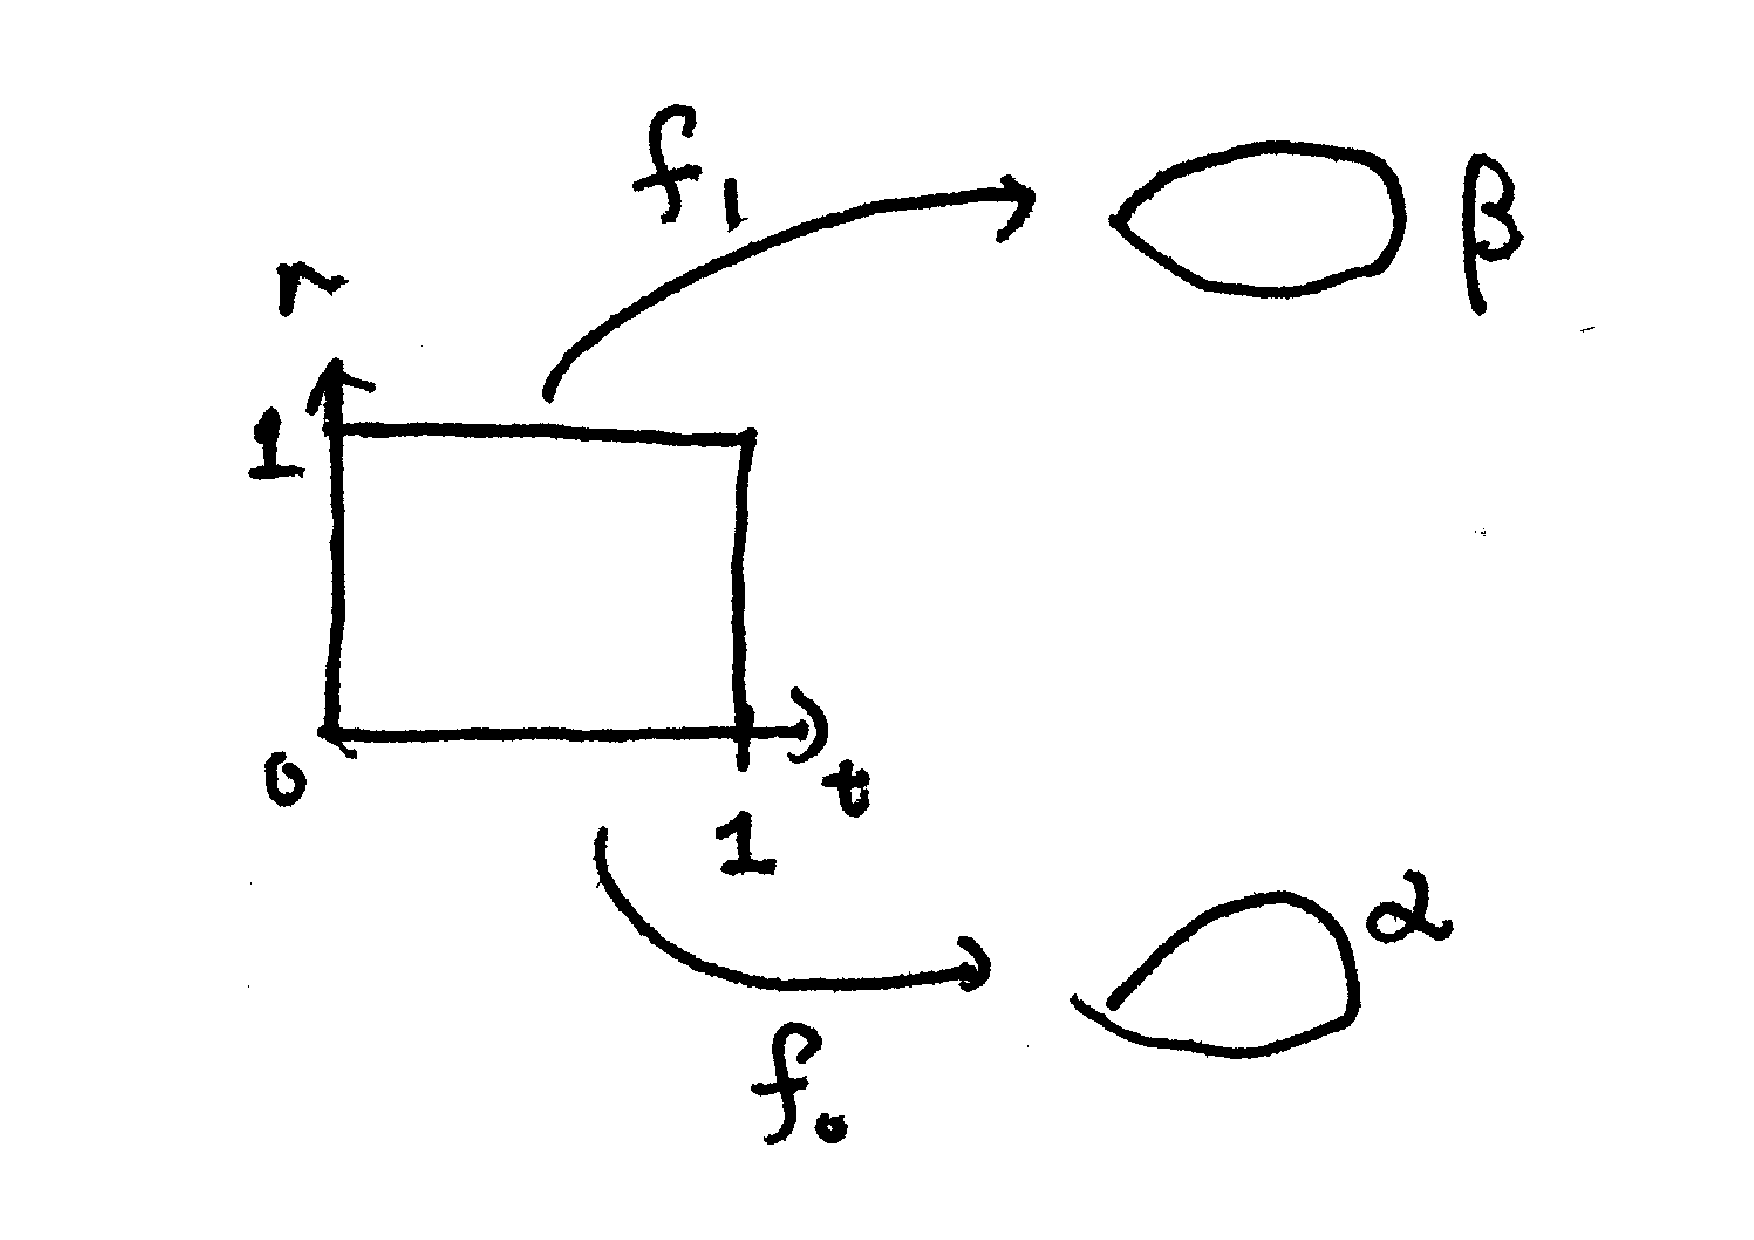
\includegraphics[width=0.6\linewidth]{pics/homotopy-for-loops.pdf}
    \caption{Homotopy for loops}
\end{figure}
This relation can be generalized to any continuous maps:
\begin{defi}[Homotopic]
\nomenclature{Homotopic}{\nomrefpage.}
    Let $f,g: X \to Y$ be continuous maps. Then $f$ is homotopic to
    $g$ if there exists a map $F:X \times I\to Y$ such that $F(x,O) =
    f(x)$ and $F(x,1) = g(x)$ for alt points $x\in X$.
\end{defi}

The map $F$ is called a \nomen{homotopy} from $f$ to $g$, and we write
\nomen{$f\simeq_F g$}. In addition, if $f$ and $g$ agree on some
$A\subset X$, we may wish to deform $f$ to $g$ without altering the
values of $f$ on $A$. In this case we ask for a homotopy $F$ from $f$
to $g$ with the additional property that 
\begin{equation}
    F(a,t)=f(a) \text{ for all $a\in A$, for all $t\in I$}
\end{equation}
when such a homotopy exists, we say the \nomen{$f$ is homotopic to $g$
relative to $A$} and write \nomen{$f\simeq_F g$ rel $A$}.
\begin{figure}[H]
    \centering
    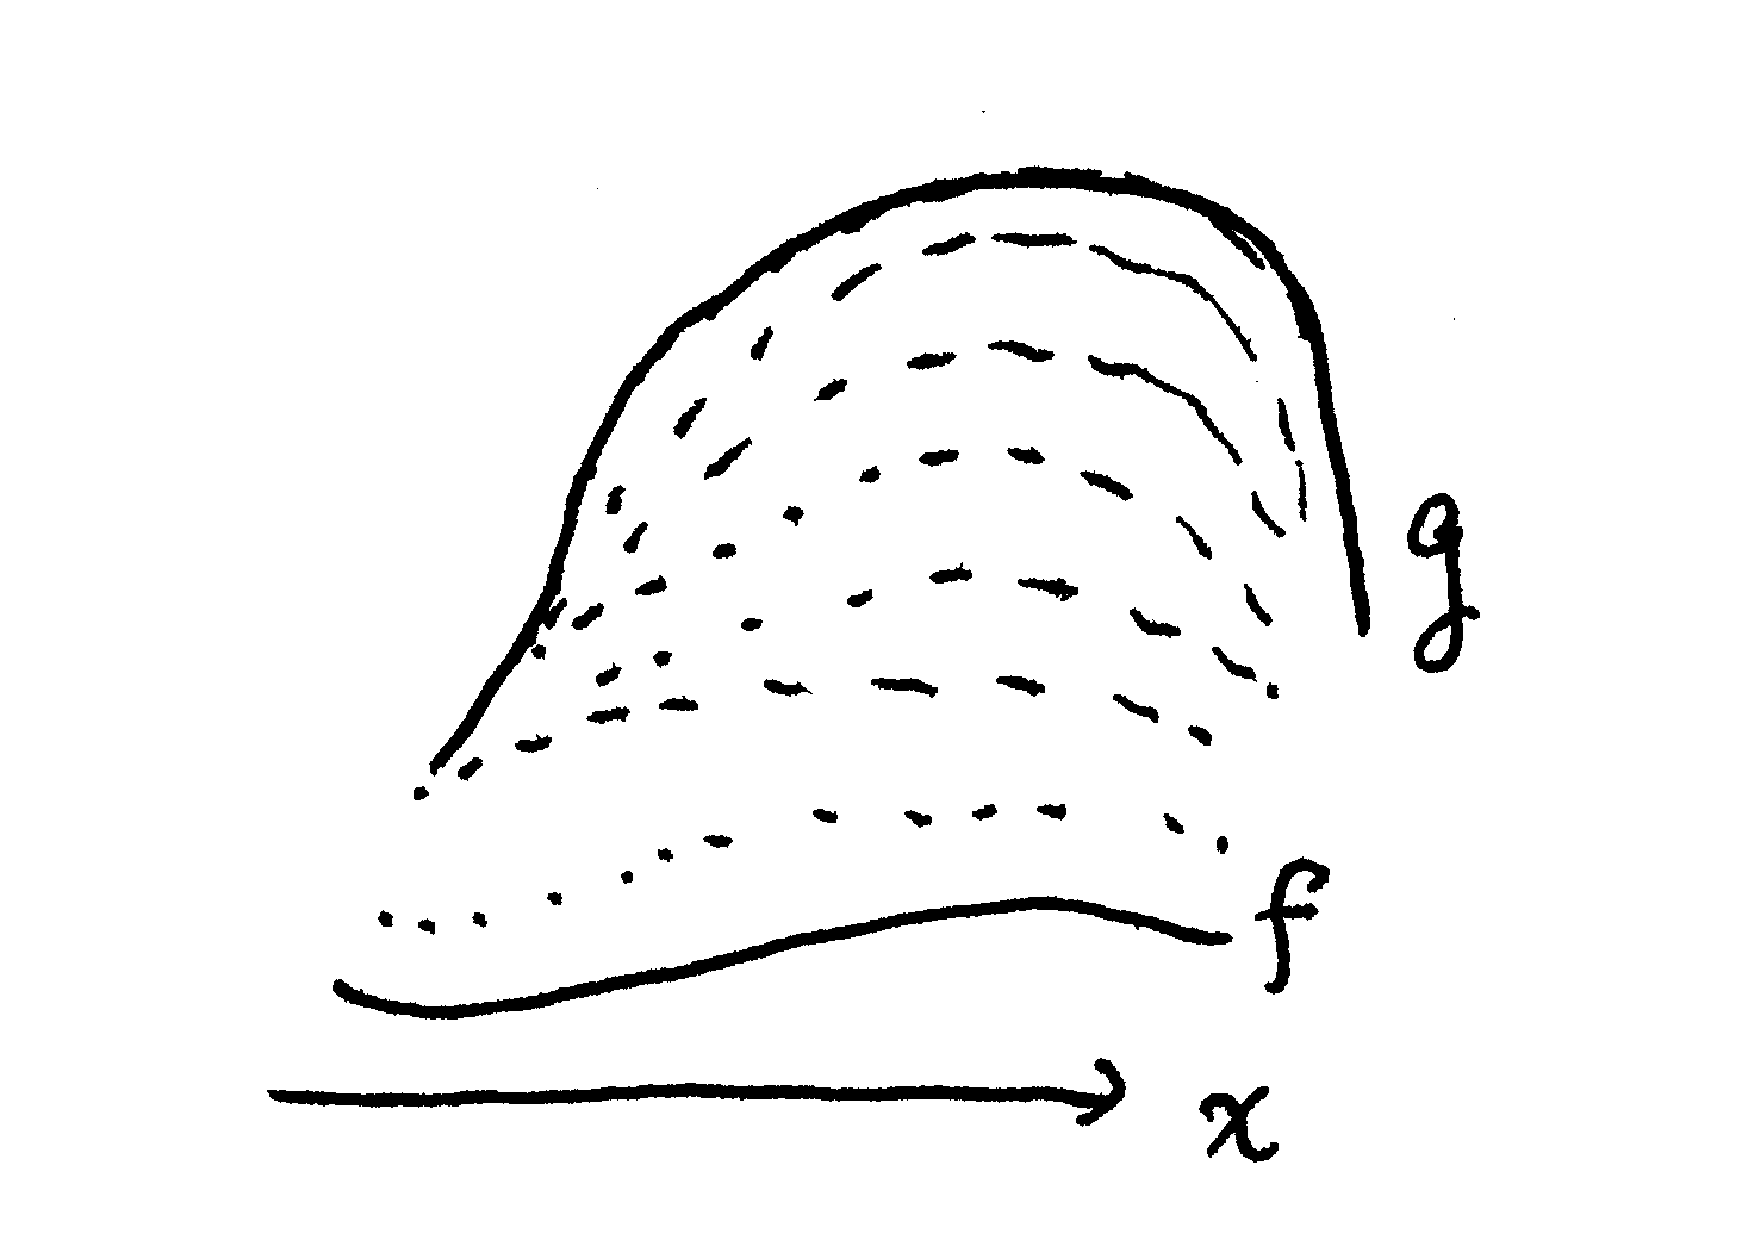
\includegraphics[width=0.5\linewidth]{pics/homotopy-schematic.pdf}
    \caption{Homotopy Scheme}
\end{figure}

When $f$ and $g$ are loops, then the homotopic relation for loops are
just saying that $f\simeq g$ rel $\{0,1\}$.

\begin{figure}[H]
    \centering
    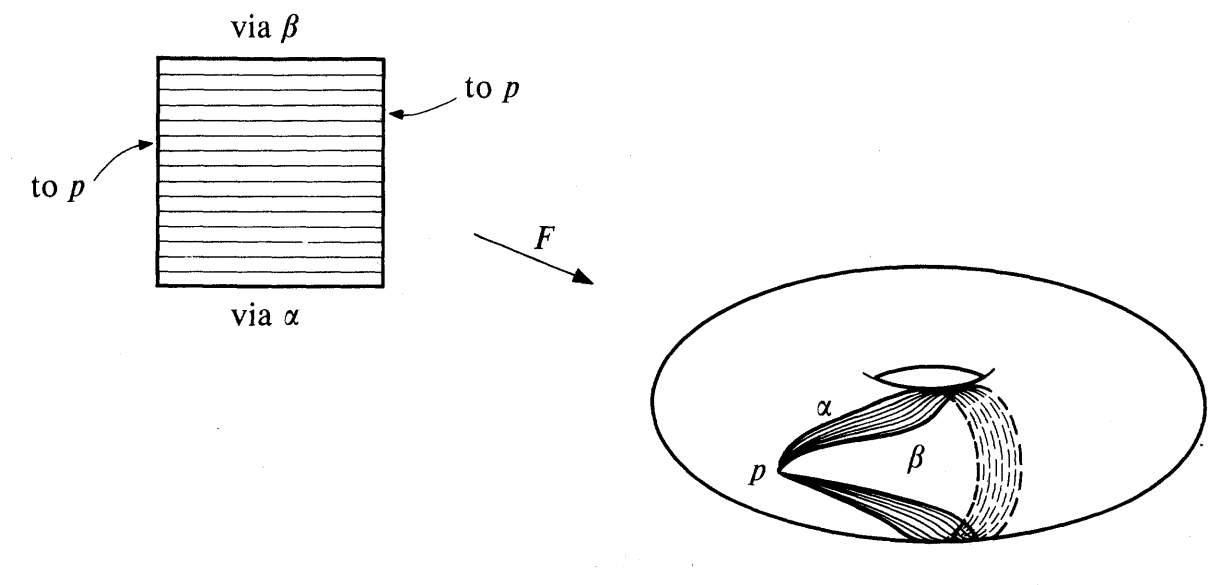
\includegraphics[width=0.7\linewidth]{pics/homotopy-for-loops-2.PNG}
    \caption{Homotopy for loops 2 (pp. 88 of \cite{book})}
\end{figure}
\begin{ex}
    The author shows on page 88 of \cite{book} that: when $C$ is a
    convex subset of a euclidean space, let $f,g:X\to C$ be continuous
    maps, then $f\simeq_F g$, where $F$ is $F(x,t)=(1-t)f(x)+tg(x)$.
    Note that if $f$ and $g$ agree on a subset $A$ of $X$, then this
    homotopy is a homotopy relative to $A$. This $F$ is called a
    \nomen{straight-line homotopy}.
\end{ex}
\begin{ex}
    Let $f,g:X\to S^n$ be continuous maps. We can take $S^n$ to be the
    unit sphere in $\mathbb{E}^{n+1}$, and think of $f,g$ as
    continuous maps into $\mathbb{E}^{n+1}$, then we may form a
    similar "straight-line homotopy" from $f$ to $g$ by:
    \begin{equation}
        F(x,t) = \frac{(1-t)f(x)+tg(x)}{||(1-t)f(x)+tg(x)||}
    \end{equation}
    Notice that the ball $B^{n+1}$ is a convex set, so the numerator
    lies inside the ball. When normalized (as in $F(x,t)$), the
    numerator is a point on the sphere.
\end{ex}
\begin{ex}
    This is example is best illustrated by pictures:
    \begin{figure}[H]
        \centering
        \includegraphics[width=0.8\linewidth]{pics/{loops-to-loops-fig5.2}.PNG}
        \caption{Loops to loops (pp. 89 of \cite{book})}
    \end{figure}
    Geometrieally, $\alpha$ winds eaeh of the segments
    $[O,\frac{1}{2}]$, $[\frac{1}{2},\frac{3}{4}]$, $[\frac{3}{4}, 1]$
    once round the eirc1e, the first two being wound in an
    anticlockwise direetion, and the third clockwise. The loop $\beta$
    simply winds the whole interval $[0,1]$ once round the circle
    anticlockwise.

    The book\cite{book} gives a homotopy $F$ between $\alpha$ and
    $\beta$ on page 89. But it is best to imagine $\alpha$ and $\beta$
    being metal coils, and this $F$ just describes the process when
    one magically strach and unfold the coil from $\alpha$ to $\beta$.

    Notice that this coil is connected head to tail, so it is
    essential that there is not pole inside the coil in order that one
    can unfold the coil from $\alpha$ to $\beta$.
\end{ex}

I think we already feel this, but the book proves it on page 90, that

\begin{lemma}
    The relation of 'homotopy' is an equivalence relation on the set
    of all maps from $X$ to $Y$.
\end{lemma}

Also
\begin{lemma}
    The relation of 'homotopy relative to a subset $A$ of $X$' is an
    equivalence relation on the set of all maps from $X$ to $Y$ which
    agree with some give map on $A$.
\end{lemma}

The book also mentions that
\begin{lemma}
    Homotopy behaves well with respect to composition of maps
\end{lemma}
which means precisely that:
\begin{itemize}
    \item If $f\simeq_F g$ rel $A$, then $hf\simeq_{hF} hg$ rel $A$.
        $$ \begin{tikzcd}[]
            A\subset X \ar[r,"f",bend left]\ar[r,"g",bend right]
                & Y \ar[r,"h"] & Z
        \end{tikzcd}$$
    \item If $g\simeq_G h$ rel $B$, then $gf\simeq_F hf$ rel $f^{-1}B$
        via the homotopy $F(x,t)=G(f(x),t)$.
        $$ \begin{tikzcd}[]
            X\ar[r,"f"] & Y \ar[r,"g",bend left]\ar[r,"h",bend right]
             & Z \\
            f^{-1}B\ar[u,phantom,"\subset"
            {anchor=south,rotate=90,left=0,near end}]
                &
            B\ar[u,phantom,"\subset" {anchor=south,rotate=90,left=0,near
            end}] & \, 
        \end{tikzcd}$$
\end{itemize}

\subsection{Construction of the fundamental group}
\label{sec:Construction-of-the-fundamental-group}

\begin{thm}
    The set of homotopy classes of loops in $X$ based at $p\in X$
    forms a group under the multiplication
    $\braket{\alpha}\cdot\braket{\beta}=\braket{\alpha\cdot\beta}$.
    The identity and inverse elements are defined on page 92 and 93 of
    \cite{book}.
\end{thm}
\begin{remark}
    Notice that the fundamental group dependes heavily on the base
    point. Especially when the space $X$ is disconnected. A natural
    intuition is that when the space is path-connected, then any two
    paths can be connected. If two points can be connected, then two
    loops based on different points can be connected. That why we have
    the following.
\end{remark}
\begin{thm}
    If $X$ is a path-connected then $\pi_1(X,p)$ $\pi_1(X,q)$ are
    isomorphic for any two points $p,q\in X$.
\end{thm}
\begin{proof}
    The proof is on page 94 of \cite{book}.
\end{proof}
\begin{defi}[$f_*$]
\nomenclature{$f_*$}{\nomrefpage.}
Suppose we have a continuous map $f:X\to Y$, $f$ can induce a map
($p\in X,q\in Y$ and $q=f(p)$).
    \begin{align}
        f_* : \pi_1(X,p) &\to \pi_1(Y,q) \\
        \braket{\alpha} &\mapsto \braket{f\circ \alpha}
    \end{align}
This map is actually a homomorphism.
\end{defi}
\begin{fact}
By construction, we have for
$$ \begin{tikzcd}[]
    X\ar[r,"f"] & Y\ar[r,"g"] & Z
\end{tikzcd}$$
\begin{align}
    (g\circ f)_* = g_* \circ f_*
\end{align}
\end{fact}
\begin{fact}
With a homeomorphism $h:X\to Y$ and the above fact, we see that
homeomorphic spaces have isomorphic fundamental groups.
\end{fact}
\subsection{Sectin 5.3}
\label{sec:Sectin-5.3}
This section calculates the following facts:
\begin{table}[H]
    \centering
    \begin{tabular}{c c c}
        \hline
        \#&  Space                           & Fundamental group \\
          \hline
        1 &  Conves subset of $\mathbb{E}^n$ & \{e\} \\
        2 &  Circle                          & $\mathbb{Z}$ \\
        3 & $S^1$                           & $\mathbb{Z}$ \\
        4 & $S^n,\, n\geq 2$                & \{e\} \\
        5 & Torus $S^1\times S^1$           & $\Z\times\Z$ \\
        6 & $P^n,, n\geq 2$                 & $\Z_2$ \\
        7 & Klein bottle                    & $\{a,b|a^2=b^2\}$ \\
        8 & Len space $L(p,q)$              & $\Z_p$ \\
          \hline
    \end{tabular}
\end{table}

\paragraph{Convex subset of $\E^n$} is on page 96 of \cite{book}.
\begin{defi}[simply connected]
\nomenclature{simply connected}{\nomrefpage.}
    A path-connected space whose fundamental group is trivial is said
    to be simply connected.
\end{defi}

\paragraph{The $n$-sphere $S^n$} is on page 99. To prove it, we
require a theorem:
\begin{thm}
    Let $X$ be a space which can be written as the union of two simply
    connected open sets $U,V$ in such a way that $U\cap V$ is
    path-connected. Then $X$ is simply connected.
\end{thm}
\begin{proof}
    Proof is on page 99 of \cite{book}. It requires the Lebesgue lemma
    \ref{lemma:lebesgue-lemma}. A picture illustrating the proof is
    provided here:
    \begin{figure}[H]
        \centering
        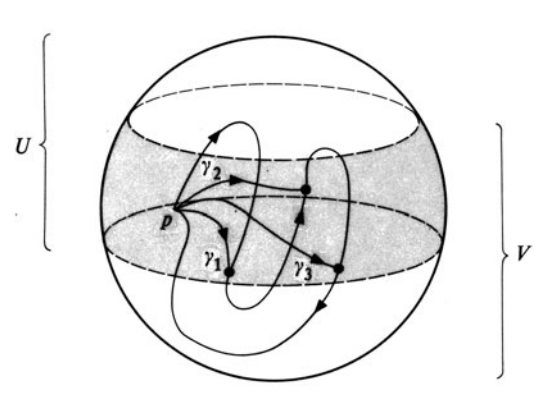
\includegraphics[width=0.6\linewidth]
        {pics/n-sphere-is-simply-con.PNG}
    \end{figure}
\end{proof}
Then, the two cover of $S^n$ are simply $U=S^n-\{x\}$ and
$V=S^n-\{y\}$, where $x,y$ are two distinct points on $S^n$. Since $U$
and $V$ are homeomorphic to $\E^n$, $S^n$ is simply-connected.

\subsection{Continued Section 5.3}
\label{sec:Continued-Section-5.3}
In this section, I will follow the lecture by professor Li Qin.
We show that
\begin{thm}
    $$\pi_1 (S^1) = \mathbb{Z} $$
\end{thm}

\begin{proof}
    Given any integer $n\in \mathbb{Z}$, we give a loop by associatng
    each $n$ 
    \begin{align*}
        \pi : \mathbb{R} \to S^1 \\
        t \mapsto e^{2\pi it}
    \end{align*}
    Define 
    \begin{align}
        \gamma_n : [0,1] \to \mathbb{R} \\
        s\mapsto n s
    \end{align}
    Then $\phi_n:= \pi\circ \gamma_n$ has the property that
    $\phi_n(0)=1$, $\phi_n(1)=1$. So we obtain 
    \begin{equation}
        \phi: \mathbb{Z} \to \pi_1  (S^1)
    \end{equation}
    Geometrically, we $\phi_n$ loops around $S^1$ in $n$ turns.

    We need to prove that $\phi$ is a isomorphism. This is done by:
    \begin{enumerate}
        \item Prove that $\phi$ is a homomorphism;
        \item Prove that $\phi$ is bijective.
    \end{enumerate}
    First,
    \begin{align*}
        \gamma_n: s \mapsto n s \\
        \gamma_m: s\mapsto m s\\
    \end{align*}
    We need
    \begin{align*}
        \braket{\pi\circ \gamma_{m+n}} =
        \braket{\pi\circ\gamma_m}\braket{\pi\circ \gamma_n}\\
    \end{align*}
    Define $\sigma:[0,1]\to \mathbb{R}$, $s\mapsto \gamma_n(s)+m$,
    this is a translation of real line. Then $\pi\circ \sigma =
    \pi\circ \gamma_n$. Then
    \begin{align*}
        \braket{\pi\circ\gamma_m}\braket{\pi\circ \gamma_n}
        = \braket{\pi\circ\gamma_m} \braket{\pi\circ\sigma}
        = \braket{\pi\circ(\gamma_m\circ \sigma)}
    \end{align*}
    $\gamma_{m+n}$ has the same domain and codomain of $\gamma_m \circ
    \sigma$, and they obviously share the same start and the same end
    point. Therefore these two path are homotopic relative to
    $\{0,1\}$.
    Therefore
    \begin{equation}
        \braket{\pi\circ \gamma_{m+n}} =
        \braket{\pi\circ(\gamma_m\circ\sigma)}
    \end{equation}
    Or
    \begin{equation}
        \phi_{m+n} = \phi_{m}\phi_n
    \end{equation}

    Second, we need to show that this map is surjective. Notice that
    $\pi:\mathbb{R}\to S^1$, $t\mapsto e^{2\pi i t}$, is like a
    projection of a circulatory path onto a circle $S^1$. This map is
    locally homeomorphic. We can find a cover of $S^1$ as the
    combination of
    \begin{align*}
        U = S^1\setminus \{-1\} \\
        V = S^1\setminus \{1\}
    \end{align*}
    Then $\pi^{-1}(V)$ are the intervals on $\mathbb{R}$ excluding the
    whole integer points. Similarly, $\pi^{-1}(U)$ are those intervals
    on $\mathbb{R}$ excluding those half-integer points. In each of those
    intervals the map $\pi$ is bijective.
    Now we need a lemma:
    \begin{lemma}[Path-lifting lemma]
        \label{thm:path-lifting-lemma-1}
        \begin{equation}
            \begin{tikzcd}[]
                \, & \mathbb{R}\ar[d,"\pi"] \\
                {[0,1]}\ar[r,"\sigma"]\ar[ru,"f"] & S^1
            \end{tikzcd}
        \end{equation}
        Assuming we have $\pi$ and $\sigma$, both are continuous maps.
        More specifically, $\sigma$ is a path in $S^1$ which begins at the
        point $1\in S^1$. Then there is a unique path $\tilde\sigma$ in
        $\mathbb{R}$ which begins at $0\in \R$ and satisfies $\pi\circ
        \tilde\sigma = \sigma$.
    \end{lemma}
    \begin{proof}
        The proof is on page 97 to 98 of \cite{book}. The class gives
        me enough intuition to understand the proof.

        The intuition is that, by Lebesgue lemma, we can divide the
        interval $[0,1]$ fine enough such that each divided part  is
        maped to only one of the cover $U$ or $V$.  We thus break a
        path $\sigma$ into small paths $\sigma_i$. Each $\sigma_i$ can
        be lifted into a path $\tilde\sigma_i$ in $\R$. But such
        lifting can be arbitrary because the inverse of $\pi$ is not a
        good function. To resolve this ambiguity, one requires the
        first path should starts with $0\in\R$, and the second should
        be continuously connected to the first, and so is the third,
        fourth, etc. This fixes the ambiguity and the paths
        $\tilde\sigma_i$ when connected give the required path
        $\tilde\sigma$.
    \end{proof}
    Note that $\tilde\sigma(0)=0$, $\tilde\sigma(1)$ is an integer.
    Now for any loop $\gamma:[0,1]\to S^1$ based at $1$, we can find a
    lifting $\tilde\gamma:[0,1]\to \mathbb{R}$ such that
    $\tilde\gamma(0)=0$,$\tilde\gamma(1)=n$, and $\gamma = \pi\circ
    \tilde\gamma$. Then $\tilde\gamma \cong \gamma_n$ rel $\{0,1\}$,
    also $\braket{\pi\circ\tilde\gamma}=\braket{\pi\circ\gamma_n}$.
    Hence for any path $\gamma$ we find a $n$ such that
    $\gamma=\phi(n)$. So \textit{the map is surjective}.



    We need another lemma to prove that it is injective.
    \begin{lemma}[Homotopy-lifting lemma]
        If $F:[0,1]\times[0,1]\to S^1$ is a map such that
        $F(0,t)=F(1,t)=1$ for $0\leq t\leq 1$, then there exists a
        unique $\widetilde F: [0,1]\times[0,1]\to \mathbb{R}$ such that
        \begin{align}
            \pi\circ \widetilde F &= F \\
            \widetilde F(0,t) &=0,\, 0\leq t\leq 1
        \end{align}
    \end{lemma}
    \begin{figure}[H]
        \centering
        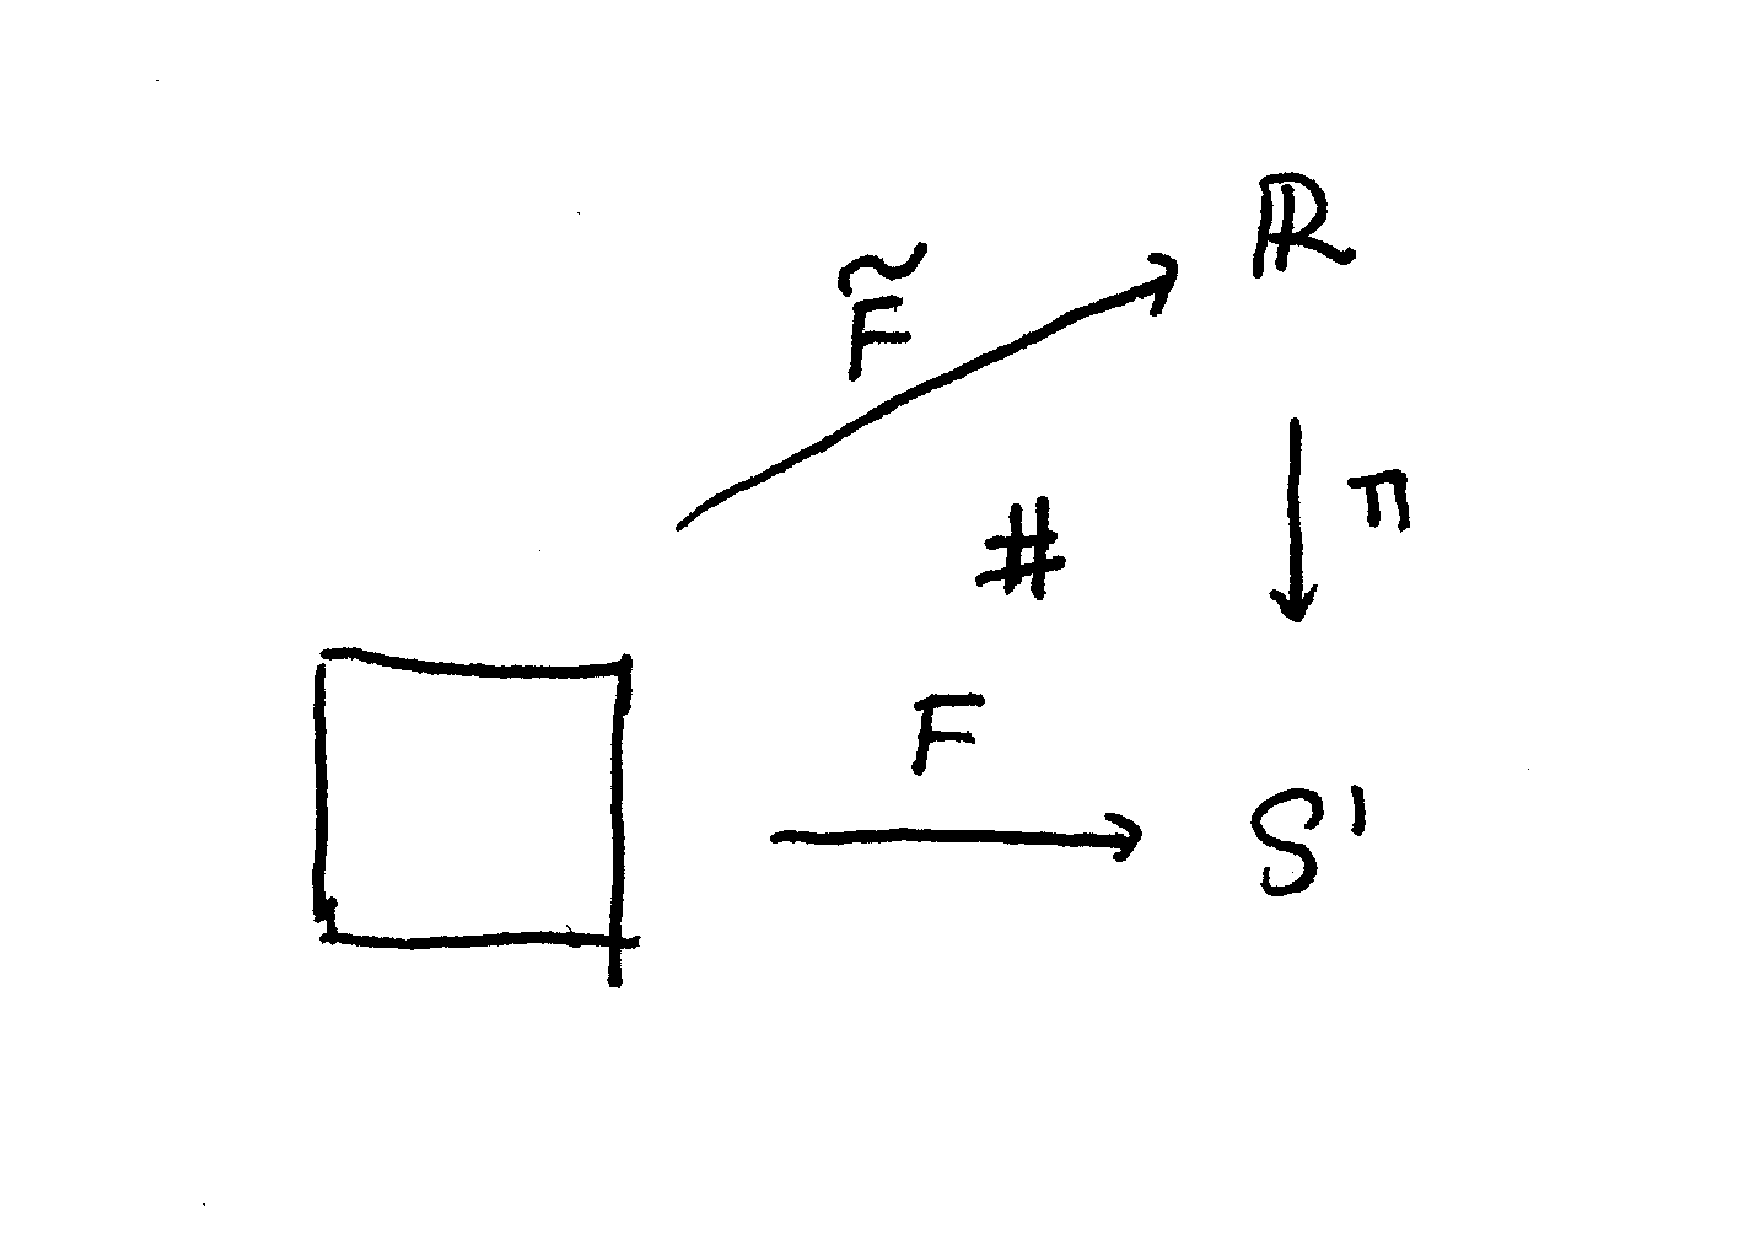
\includegraphics[width=0.5\linewidth]{pics/homotopy-lifting-1.pdf}
        \caption{Homotopy lifting lemma-1}
    \end{figure}
    \begin{proof}
        The proof is on page 98 of \cite{book}. The idea is exactly
        the same as in lemma~\ref{thm:path-lifting-lemma-1}.
    \end{proof}
    Now we proof that the map $\phi$ is injective. Suffice to prove
    that $\Ker(\phi)$ is trivial. Suppose $\phi(n)=\pi\circ \gamma_n$
    is homotopic to the constant loop. Then choose a homotopy $F$
    from $\pi\circ\gamma_n$ to the constant loop. By the
    homotopy-lifting lemma we can find $\widetilde F: [0,1]\times[0,1]\to
    \mathbb{R}$ such that $\pi\circ \widetilde F = F$. Also
    $\widetilde F(0,t)=0$.
    We can find the vertical bottom is $0$ and verticl top is
    $\gamma_n$. Right line is integers and can only be $0$. 
    \begin{figure}[H]
        \centering
        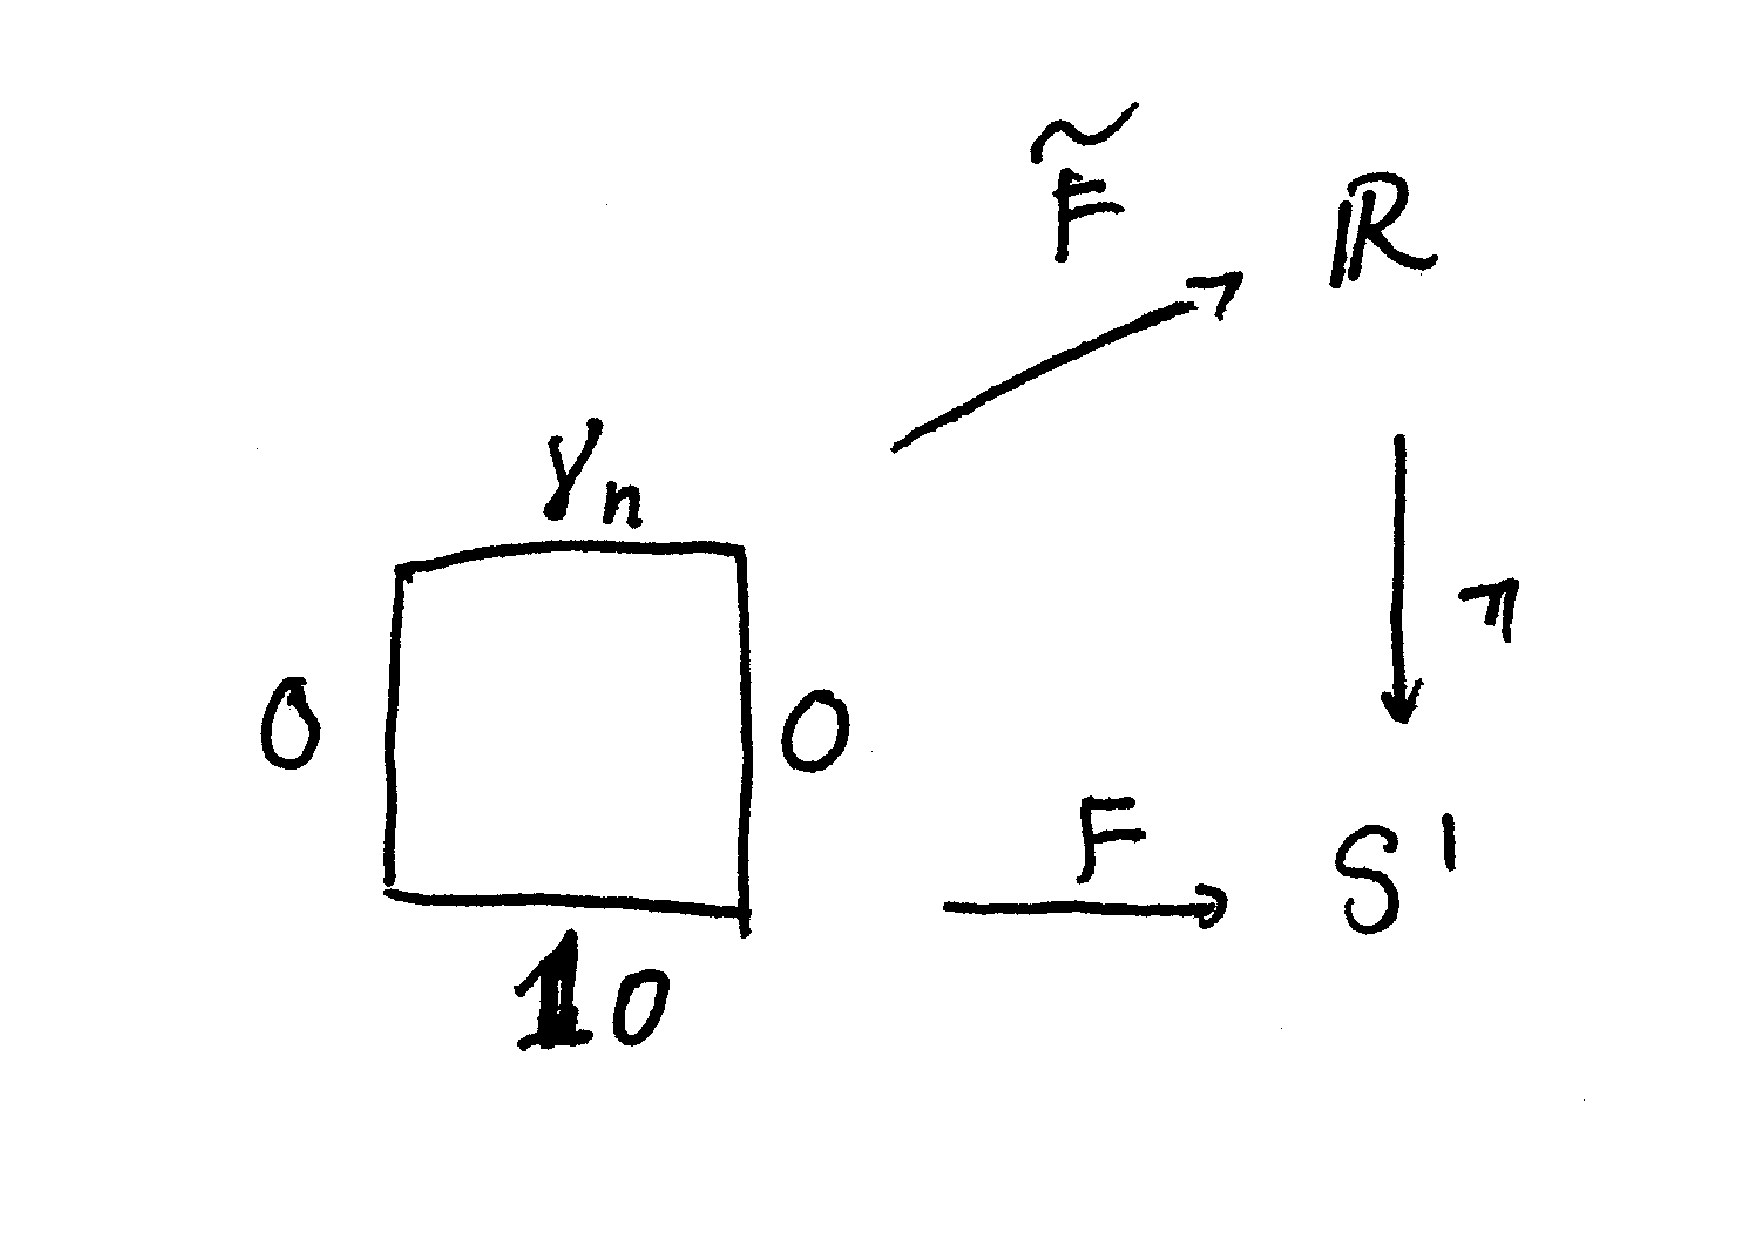
\includegraphics[width=0.6\linewidth]{pics/homotopy-lifting-2.pdf}
        \caption{Schematic Draft}
    \end{figure}
    Hence $\gamma_n$ starts at $0$ and ends at $0$.  One can find that
    $\gamma_n\cong 0$. This completes the proof of injectivity. Hence
    completes the whole proof.
\end{proof}

We have an application,
\begin{thm}[Brouwer Fixed Point theorem]
    A contiuous map $f:B^2\to B^2$ ($B^2:2D$-closed dicks) must have a
fixed point. That is, $\exists x\in B^2$ such that $f(x)=x$.
\end{thm}
\begin{proof}
    Assuming that this theorem is false, that is $\forall x\in B^2$,
    $x\neq f(x)$, then we have a straight path from $f(x)$ to $x$. We can
    extends this path to cuts the boundary of $B^2$ at $h(x)$. This is
    for all $x\in B^2$, hence we have a map $h: B^2 \to S^1$. Also,
    $h|_{S^1}$ is obvious an identity map. But $S^1$ can be included
    inside $B^2$, so we have:
    \begin{equation}
        S^1 \to B^2 \to S^1
    \end{equation}
    Hence we have a series of homomorphism of fundamental groups:
    \begin{equation}
        \pi_1 (S^1) \to \pi_1 (B^2) \to \pi_1(S^1)
    \end{equation}
    and the composite is identity map. But observe that $B^2$ is a
    convex set and hence its fundamental group is trivial. But $S^1$
    has non-trivial fundamental group. It is then impossible to form
    such a chain of homomorphism whose product is identity map.
    Contradiction!
\end{proof}
\begin{remark}
    This theorem can be extended to higher dimensional case. But the
    proof cannot be the same because for higher dimension $\pi_1(S^n)$
    is no longer non-trivial.
\end{remark}

Another application, which we need a theorem to help:
\begin{thm}
    \begin{equation}
        \pi_1 (X\times Y, (x_0,y_0)) = \pi_1 (X,x_0) \otimes \pi_1
        (X,y_0)
    \end{equation}
\end{thm}
\begin{proof}
    We use the projection maps: $P_1$ and $P_2$.
    Then, the map
    \begin{align*}
        (P_1)_*: \pi_1 (X\times Y) \to \pi_1(X) \\
        (P_2)_*: \pi_1 (X\times Y) \to \pi_1(Y)
    \end{align*}
    and their composition formed into
    \begin{align*}
        \braket{\alpha}\mapsto
        (\braket{P_1\circ\alpha},\braket{P_2\circ\alpha})
    \end{align*}
    this map is surjective, injective, and is homomorphism.
    The detail can be found on page page 101 of \cite{book}.
\end{proof}

\begin{fact}
By this theorem, the two objects $S^2$ and $S^1\times S^1$ is not
homeomorphic, since their fundamental groups are not the same (the
former is trivial and the later is $\mathbb{Z}\times\mathbb{Z}$).
\end{fact}

% TODO homework: pro 13 of page 95.

\subsection{Homotopy Type}
\label{sec:Homotopy-Type}

Notice that a homeomorphic map will make two space have the same
fundamental group, but two space having the same fundamental group may
not be homeomorphic. For example, the plane and the $S^2$ both have
the same $\pi_1=\{e\}$, but the plane is not compact while the
$2$-sphere is, i.e. they are not homeomorphic.

Notice also that homeomorphic requires $fg^{-1}=\id$, whereas under
homotopic relation, we may require $fg^{-1}\cong\id$. Therefore we may
also define a new type of relationship between topological spaces:

\begin{defi}[Homotopy type]
\nomenclature{Homotopy type}{\nomrefpage.}
    Two spaces $X$ and $Y$ have the same homotopy type, or they are
    homotopy equivalent, if there exist maps:
    $$ \begin{tikzcd}[]
        X\ar[r,"f",bend left] & Y\ar[l,"g",bend left]
    \end{tikzcd}$$
    such that $g\circ f\cong \id_X$, and $f\circ g\cong\id_Y$.
\end{defi}
\begin{fact}
This relationship must be an equivalence relation on topological
spaces, as confirmed by lemma (5.16) on page 103 of \cite{book}.
\end{fact}
\begin{remark}
    The topological spaces $X$ and $Y$ are not necessarily
    path-connected! But we have:
\end{remark}
\begin{fact}
    If $X$ and $Y$ have the same homotopy type then $X$ is
    path-connected if and only if $Y$ is path-connected. (This is
    noted in a footnote on page 107 of \cite{book}.)
\end{fact}
\begin{defi}[Deformation retraction]
\nomenclature{Deformation retraction}{\nomrefpage.}
    Let $A$ be a subspace of $X$. Let a homotopy $G:X\times I\to X$ which
    is relative to $A$ and for which
    $$ \begin{cases}
        G(x,0)=x & \\
        G(x,1)\in A
    \end{cases}$$
    for all $x\in X$. Then $G$ will be called a deformation retraction
    of $X$ onto $A$.
\end{defi}
\begin{remark}
    If there is a deformation retraction of $X$ onto $A$, then of
    course $X$ and $A$ have the same homotopy type.
\end{remark}
Following is an example of a deformation retraction:
\begin{figure}[H]
    \centering
    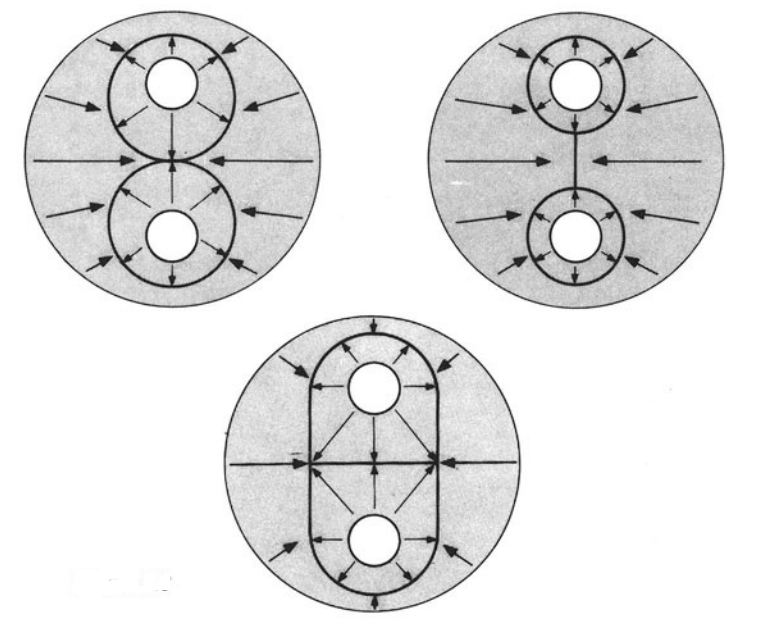
\includegraphics[width=0.8\linewidth]{pics/deformation-retraction.PNG}
    \caption{Three Deformation Retractions (from \cite{book})}
\end{figure}

Exmaples from the book:
\begin{ex}
    Homeomorphic spaces have the same homotopy type.
\end{ex}
\begin{ex}
    Any convex subset of a euclidean space is homotopy equivalent to a
    point.
\end{ex}
\begin{ex}
    $\E^n\setminus \{0\}$ has the homotopy type of $S^{n-1}$. This is
    shown on page 104 of \cite{book}, and is illustrated there by:
    \begin{figure}[H]
        \centering
        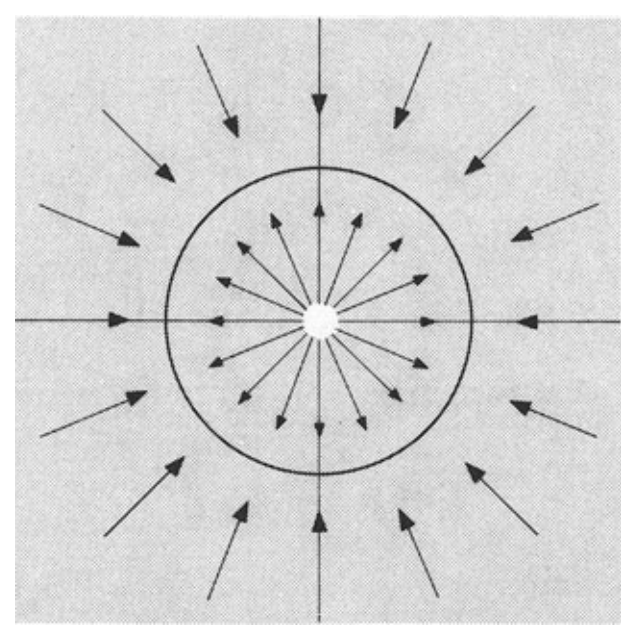
\includegraphics[width=0.6\linewidth]{pics/En-0-and-S-n-1.PNG}
        \caption{$E^n\setminus\{0\}$ and $S^{n-1}$}
    \end{figure}
\end{ex}

\begin{thm}
    If $f\cong_F g:X\to Y$ then $g_*:\pi_1(X,p)\to \pi_1(Y,g(p))$ is
    equal to the composition
    \begin{equation} \begin{tikzcd}[]
        \pi_1(X,p)\ar[r,"f_*"]&\pi_1(Y,f(p))\ar[r,"\gamma_*"]
            &\pi_1(Y,g(p))
    \end{tikzcd} \end{equation}
    where $\gamma$ is the path joining $f(p)$ to $g(p)$ in $Y$ defined
    by $\gamma(s)=F(p,s)$.
\end{thm}
\begin{proof}
    Proof can be found on page 105 of \cite{book}.
\end{proof}

\begin{thm}
    If two \hl{path-connected} spaces are of the same homotopy type, then
    they have isomorphic fundamental group.
\end{thm}
\begin{proof}
    Proof can be found on page 106 of \cite{book}. Here's a note using
    the notation in that book:
    $$ \begin{tikzcd}[]
        X\ar[r,"f",bend left] & Y\ar[l,"g",bend left]
    \end{tikzcd}$$
    It should be noticed that the continuity allows one to identify the
    diagram:
    $$ \begin{tikzcd}[]
        \pi_1(X,p)\ar[r,"(gf)_*"]\ar[rr,"\id",bend right]
            &\pi_1(X,gf(p))\ar[r,"\gamma^{-1}_*"]
            &\pi_1(X,p)
    \end{tikzcd} $$
    with the diagram:
    $$ \begin{tikzcd}[]
        \pi_1(X)\ar[r,"(gf)_*"]\ar[rr,"\id",bend right]
            &\pi_1(X)\ar[r,"\gamma^{-1}_*"]
            &\pi_1(X)
    \end{tikzcd} $$
\end{proof}

\begin{fact}
Using the above fact, we can find that the M\"obius strip, the cylinder,
the punctured plane $\E^2\setminus\{0\}$, and the solid torus, all
have the homotopy type of a circle $S^1$, and consequiently have $\Z$
as fundamental group.
\end{fact}
\begin{fact}
    Also, $\E^n\setminus\{0\}$ deformation-retracts onto $S^{n-1}$ and
    is therefore a simply connected space when $n\geq 3$.
\end{fact}

\begin{defi}[Contractible]
\nomenclature{Contractible}{\nomrefpage.}
    A space $X$ is called contractible if the identity map $\id_X$ is
    homotopic to the constant map at some point of $X$.
\end{defi}
\begin{thm}$ $

    \begin{enumerate}
        \item A space is contractible if and only if it has the
            homotopy type of a point.
        \item A contractible space is simply connected.
        \item Any two maps into a contractible space are homotopic.
        \item If $X$ is contractible, then $\id_X$ is homotopic to the
            constant map at $x$ for any $x\in X$.
    \end{enumerate}
\end{thm}
\begin{ex}
    Here is a contractible space that is really hard to imagine. It is
    called the topologist's dunce hat. It is formed by identifying the
    sides of a triangle in the manner indicated in the following
    figure:
    \begin{figure}[H]
        \centering
        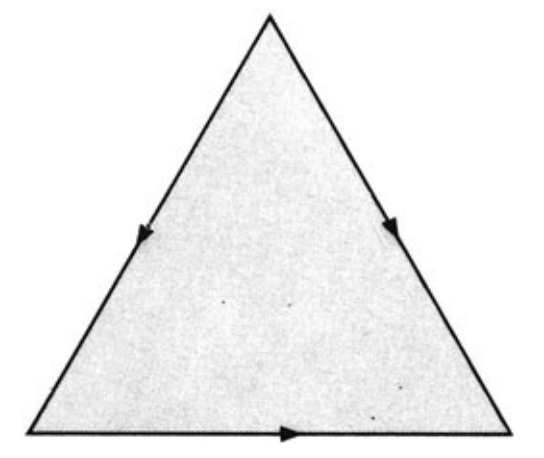
\includegraphics[width=0.4\linewidth]{pics/topo-dunce-hat.PNG}
        \caption{Topologist's dunce hat}
        \label{fig:topo-d-hat}
    \end{figure}
    You may imagine identifying a pair of sides, then identify the
    identitied edge to the resting side. The direction for identifying
    is really important.
    This space is contractible. Despite some hard words said by the
    book, it is really simple to see on figure~\ref{fig:topo-d-hat}.
    Draw any loop on it and shrink it. Noticing that all edges are
    identified, though in some odd direction.
\end{ex}

\begin{remark}
    An identity function $\id_X$ on a contractible space $X$
    is homotopic to constant function $\id_p$ on a point $p\in X$. But
    this homotopy may not keep the point $p$ fixed. That is, we do not
    necessarily have $\id_X\cong\id_p$~rel $p$.

    An example on page l08 of \cite{book}. In a space called
    the topologist's comb:
    \begin{align*}
        K &= \{\frac{1}{n}|n\in\N\setminus\{0\}\} \\
        \text{comb space}&=(\{0\} \times [0,1] ) \cup (K \times [0,1]) \cup ([0,1] \times \{0\})
    \end{align*}
    \begin{figure}[H]
        \centering
        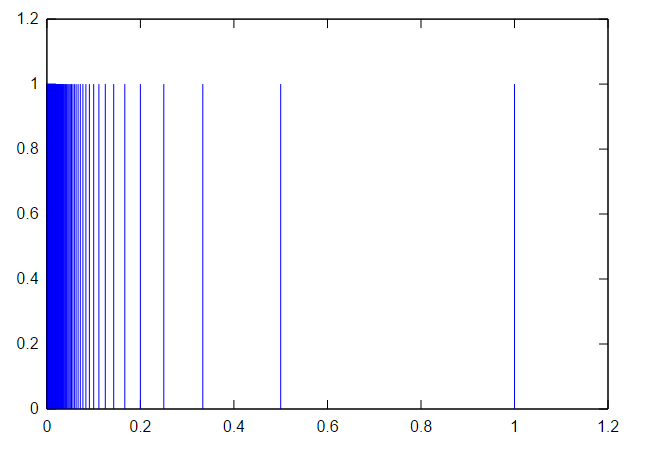
\includegraphics[width=0.6\linewidth]{pics/comb-space.PNG}
        \caption{Topologist's Comb (from Wikipedia)}
    \end{figure}
    We cannot continuously defrom the identity function $\id_X$ to the
    constant function on $p=(0,1)$. Intuitively, there are infinite
    points around $p$ that are infinitesimally close to it. But the
    identity function must shrink from all these infinite points to
    the base line $[0,1]$ without afftecting the value on $p$. This
    sounds unlikely.

    Analytically, the argument is provided by
    \href{http://math.stackexchange.com/users/172604/pedro}{Pedro} in
    his Math.SE
    \href{http://math.stackexchange.com/a/952989/184811}{post}:

    \begin{myquote} \enquote{
        \textbf{Idea:} Take the sequence $x_n=(\frac{1}{n},1)$, it
        converges to $x_0$. If existed such homotopy $H(x,t)$ then the
        sequences $H(x_{n},t)$ would still converge to $x_{0}$.

        You have for each neighborhood $U$ of $x_0$ a number
        $N_{(U,t)}$ and $\epsilon_{(U,t)}$ such that $H(x_n,s)\in U$
        for $n>N_{(U,t)}$ and $|t-s|<\epsilon_{(U,t)}$.

        Covering the interval $I$ with
        $(t-\epsilon_{(U,t)},t+\epsilon_{(U,t)})$ and taking a finite
        subcover you obtain a number $N$ such that $H(x_n,t)\in U$ for
        any $n>N$ and $t\in[0,1]$.

        Now you can use disconnectedness of a small neighborhood to
        show that the homotopy can't take the elements of the sequence
        to $x_0$. 
    } \end{myquote}
\end{remark}
